\chapter{Judges and Officials Rules}

\section{Performance Set-Up}
\oldrule{5.4}
Competitors are allowed a maximum of two minutes to set up their unicycles and props in the performing area.
Competitors who take too long risk being disqualified.
An extension of the set-up time can be given only by the Chief Judge and must be requested in advance.
Competitors must show a legitimate need when requesting more time, such as numerous props or complicated special effects.

\section{Interruption Of Judging}
\oldrule{5.5}
An interruption of judging can result from material damage, injury or sudden illness of a competitor, or interference with a competitor by a person or object.
If this happens, the Chief Judge determines the amount of time left and whether any damage may be the fault of the competitor.
Re-admittance into competition must happen within the regulatory competition time.
If a routine is continued and the competitor was not at fault for the interruption, all devaluations coming forth from the interruption will be withdrawn.

\section{Freestyle Judging Panel \label{sec:freestyle_judging-panel}}
\oldrule{5.9}
There are five (or more) judges each of Technical and Presentation for Age Group competitions; five (or more) judges each of Technical and Presentation for Jr. Expert and Expert competitions (including Group).
All judges must attend a workshop provided as part of the convention schedule before the start of the Freestyle competitions.
Exceptions to workshop attendance are granted by the Chief Judge if judging rules have not changed since the previous judging experience and the judge has high Accuracy Scores.
Unless otherwise noted, judges at a Unicon must either speak English or have translation assistance for the specified language while judging.
Judges at other unicycle conventions should speak the dominant language of that convention or have translation assistance.

Judges' names must be provided to the Chief Judge (via email, FAX, or postal mail) by at least one month prior to the start of the unicycle convention and include the number of freestyle conventions where they have been a competitor, judge, or simply in the audience.
See section \ref{subsec:freestyle_judging-panel_nominating-freestyle-judges} for description of which teams/countries are required to provide judges.
Judges must be at least 15 years of age at the start of the event.
Judges are recommended to be a current freestyle competitor, a former freestyle competitor, an active coach of freestyle routines, a proven judge at prior competitions, or an avid spectator who has observed many freestyle routines.
Details about the Standard Skill judging panel are covered in section \ref{sec:freestyle_std-judging-panel}.

\subsection{Selecting Judges \label{subsec:freestyle_judging-panel_selecting-judges}}
\oldrule{5.9.1}
A person should not judge an event if he or she is:
\begin{itemize}
\item A parent, child or sibling of a rider competing in the event.
\item An individual or team coach, manager, trainer, colleague who is member of the same club specified in the registration form, colleague's family etc.
of a rider competing in the event.
\item More than one judge from the same family judging the same event at the same time.
\end{itemize}
If the judging pool is too limited by the above criteria, restrictions can be eliminated starting from the bottom of the list and working upward as necessary only until enough judges are available.
If there are some candidates who have the same level of restrictions and judging score, their agreement about publishing the results need to be considered.
The eliminations must be agreed upon by the Chief Judge and Artistic Director, or next-highest ranking artistic official if the Chief Judge and Artistic Director are the same person.

\subsection{Assignment Of Age Group Judges}
\oldrule{5.9.2}
Judges will be chosen from the list of judges as provided in section \ref{subsec:freestyle_judging-panel_nominating-freestyle-judges}.
Judges who are competing in the event just before or just after the current category are strongly suggested to be eliminated from the list.
Judges will also be eliminated from the list for the current category as described in section \ref{subsec:freestyle_judging-panel_rating-judge-performance}.
The final selection of judges will be chosen based on their accuracy scores from the remaining list.

\subsection{Assignment Of Expert (And Junior Expert) Judges \label{subsec:freestyle_judging-panel_assignment-of-expert-judges}}
\oldrule{5.9.3}
Assignments for Expert and Jr. Expert judges will be made by the Chief Judge using the most qualified of all judges available.
Qualifications are determined in the following order of importance: 
\begin{itemize}
\item Highest judging accuracy scores obtained while judging age group (age groups judges must have a minimum of five entrants) or other Jr. Expert and Expert events.
\item Greatest amount of Jr. Expert and Expert judging experience.
\item Greatest amount of international judging experience.
\item Greatest number of Freestyle competition experienced (viewed, judged, or as a competitor).
\end{itemize}
Judges who are competing in the event just before or just after the current category are eliminated from the list.
Judges will also be eliminated from the list for the current category as described in section \ref{subsec:freestyle_judging-panel_selecting-judges}.
Judges will also be eliminated from the list if they exhibit Judging weaknesses during their Age Group judging as described in Section \ref{subsec:freestyle_judging-panel_rating-judge-performance}.
At Unicons, if more than five judges each of Technical and Presentation remain, judges who have not judged at a previous Unicon will be removed from the list.
If there are still more than five each then the final list of judges for the category will be chosen by accuracy scores as defined in section \ref{subsec:freestyle_judging-panel_calculating-accuracy-scores}.

\subsection{Judging Panel May Not Change}
\oldrule{5.9.4}

The individual members of the judging panel must remain the same for entire age groups; for example one judge may not be replaced by another except between age groups.
In the event of a medical or other emergency, this rule can be waived by the Chief Judge.

\subsection{Rating Judge Performance  \label{subsec:freestyle_judging-panel_rating-judge-performance}}
\oldrule{5.9.5}

Judges are rated by comparing their scores to those of other judges at previous competitions.
Characteristics of Judging Weaknesses
\begin{itemize}
\item \textbf{Excessive Ties:} A judge should be able to differentiate between competitors.
Though tying is most definitely acceptable, excessive use of tying defeats the purpose of judging.
\item \textbf{Group Bias:} If a judge places members of a certain group or nation significantly different from the other judges.
This includes a judge placing members significantly higher or significantly lower (a judge may be harsher on his or her own group members) than the other judges.
\item \textbf{Inconsistent Placing:} If a judge places a large number of riders significantly different from the average of the other judges.
\end{itemize}

\subsection{Re-Instating Judges}
\oldrule{5.9.6}

If a judge has been labeled as having a Judging Weakness, they may have a chance to be re-instated on the list by:
\begin{itemize} 
\item Discuss with the Chief Judge the scores that were Tied, Biased, or Inconsistent.
\item Practice judge on at least two categories with at least 4 competitors.
\end{itemize}
If the practice judging shows no further examples of Judging Weakness, they may be reinstated on approval by the Chief Judge and Artistic Director.
If the Chief Judge and Artistic Director are the same person, then the next highest-ranking official must agree to the reinstatement.

\subsection{Calculating Accuracy Scores \label{subsec:freestyle_judging-panel_calculating-accuracy-scores}}
\oldrule{5.9.7}

The Chief judge should decide to replace a judge if he/she shows signs of weakness.
To find the right decision, the chief judge may use heuristics, statistical analytics, etc. as indicators.

\subsection{Nominating Freestyle Judges \label{subsec:freestyle_judging-panel_nominating-freestyle-judges}}
\oldrule{5.9.8}

Parties (Countries/Clubs) that participate at competitions must nominate judges in relation to the number of Freestyle participants they send (see table below). 
After registration finishes, the chief judge will send a request to all parties.
The request contains the compiled number of minimum judges per party and a question to nominate the candidates.
Judge nominations include the experience of the judges (such as previous competitions, how long he/she has been judging, agegroup/expert judging or other relevant qualifications such as educations).

\begin{tabular}{|l|l|}
\hline
\textbf{Number of Participants per Party} & \textbf{Minimum Number of Judges per Party} \\
\hline
$<$5 & 0 \\
\hline
5-10 & 2 \\
\hline
11-20 & 3 \\
\hline
21-30 & 4 \\
\hline
$>$30 & 5 \\
\hline
\end{tabular}

\subsection{Not Providing Judges}
\oldrule{5.9.9}

At Competitions, parties that are unable to provide their required number of judges (either Group or Individual/Pairs) may have their competitors removed from that competition.
Exceptions will be granted on a special basis with a letter to the Chief Judge, Artistic Director, and Convention Director. 
\textbf{Note:} A party that isn’t able to nominate their minimum judges can ask a party that has more than the required number of minimum judges to nominate their additional judges as their own.

\subsection{Judges Workshop}
\oldrule{5.9.10}

The hosts of the convention must provide for a judge's workshop at least 24 hours prior to the start of the Freestyle competition.
A minimum of 3 hours must be set aside, in a classroom or similar environment.
If possible, it is strongly recommended to have more than one workshop to accommodate schedules.
Variations on this can be approved by the Chief Judge.
Workshop schedule(s) must be announced to all judges at least three weeks prior to the start of the competition.

Judges should have read the rules prior to the start of the workshop.
The workshop will include a practice judging session.
Each judge will be required to sign a statement indicating they have read the rules, attended the workshop, agree to follow the rules, and will accept being removed from the list of available judges if their judging accuracy scores show Judging Weaknesses.

\section{Scoring}
\oldrule{5.10}
In all events except Standard Skill, the scores of each judge are transferred into placing points, which represent the ranking of each competitor by that judge.
The highest scoring competitor gets 1 placing point, the next one gets 2, and so on.

\textbf{Note:} The ranking number, or highest placing point available for a competitor depends on the number of entries in that category.
If two or more competitors have the same score, they are awarded equal portions of the total number of placing points available for the places they occupy in the ranking.

\textbf{Example:} Seven competitors.
Four of them tie for 2nd place.
7th place gets 7 points, 6th place gets 6 points, and 1st place gets 1 point.
For the other four competitors, add up the other placing points numbers: $2+3+4+5=14$.
Divide this by the number of competitors (4) to get 3.5 placing points each.

\subsection{Removing The High And Low}
\oldrule{5.10.1}
After determining placing points as above, discard the highest and lowest placing score for each rider.
If Rider A has scores of 1,2,1,3,2, take out one of the ones, and the three.
Then Rider A has 1,2,2, for a total of 5.
If Rider B has scores of 2,2,2,2,2, he will end up with 2,2,2, a total of 6.
The winner is the competitor with the lowest total placing points score after the high and low have been removed.

\subsection{Ties}
\oldrule{5.10.2}
If more than one competitor has the same placing score after the above process, those riders will be ranked based on their placing scores for Technical.
The scoring process must be repeated using only the Technical scores for the tied riders to determine this rank.
High and low placing scores are again removed in the process.
If competitors' Technical ranking comes out equal, all competitors with the same score are awarded the same place.


\subsection{Competitor and Judging Forms}
\oldrule{5.37.4}
If available to the organizers, a computer database should be used to generate forms for both the competitor and the judges, and then be used to calculate the scores.
Either the Writing Judge Form or the traditional Standard Skill Form is required for judging.
The other forms are suggested to help both the competitors and judges.
Suggested forms are: 
\begin{itemize}
\item \textbf{Competitor Form:} Skill Order, Figure number and letter, Description, Score, and Skill Definition.
\item \textbf{Standard Skill Form:} Skill Order, Figure number and letter, Description, Score, and areas to mark 50/100\% technical devaluations and the ~ / + 0 execution devaluations.
An area at the bottom should be included to write in the names of the three judges.
An area at the bottom should also be included to help in manual scoring of the routines.
\item \textbf{Writing Judge Form:} Skill Order, Figure number and letter, Description, Score, and areas to mark 50/100\% technical devaluations and the ~ / + 0 execution devaluations.
An area at the bottom should be included to write in the names of the three judges.
\item \textbf{Difficulty Judge Form:} Skill Order, Figure number and letter, Description, Score, Skill Definition, and area to mark 50/100\% technical devaluations.
The addition of the Skill Definition can help the judge if there is clarification needed for the correct execution of the skill.
\item \textbf{Execution Judge Form:} Skill Order, Figure number and letter, Description, Score, and area to mark the ~ / + 0 execution devaluations.
\end{itemize}

All three judging forms should have grey shading to indicate the relative speed of the skills.
No shading would indicate a slower skill (typically all riding skills), a light grey indicates skills that are quicker than the riding skills (most of the counted short skills), and a dark grey indicates skills that are very quick.
This will help the judges estimate how quickly they must watch for new skills.

\chapter{2013 Standard Skill Judging}

\section{Judging Panel \label{sec:freestyle_std-judging-panel}}
\oldrule{5.38}
There will be 1 Chief Judge, 2 Difficulty Judges, 2 Execution Judges, 2 Writing Judges, and 1 Timer.
The judging panel will be divided into two judging units, each consisting of one Difficulty, one Execution, and one Writing Judge.
The judges will be appointed to the functions Writer, Execution, and Difficulty, respectively in order of their experience.
At Unicons, all judges for the Expert groups must have previous Unicon judging experience.

\section{Operation Of The Judges}
\oldrule{5.39}

While the Difficulty and Execution Judges watch the routine, the Writing Judge reads the names of the figures from the list.
The Difficulty Judge indicates if a skill was fully completed, or the reduction percentage if it was not.
The Execution Judge indicates the execution mistakes using symbols, as described below.
The Writer writes down the verbal remarks of both judges on the judging sheet.
For this reason, the Writer is seated between the other two judges.
The position of the judging table must be so that all judges have a clear view of the entire riding area.
There must be enough space between the two judging units to ensure their working independently of each other.

A video of the performance may be reviewed if there are discrepancies in judge scores, or if a judge is in doubt about one or more of his/her scores.
When time allows, video can be reviewed by approval of the Chief Judge.
The Chief Judge should prearrange for routines to be recorded, but this is not a mandatory requirement.

Alternatively, to speed up the competition and judging, video cameras should be used to record the competition.
There must be at least two cameras, one on each of the two corners.
A third camera in the center is also good for a backup.
The recordings should be downloaded to a computer in approximately groups of ten competitors.
The judges will all be in a separate viewing area to watch the videos and make their scores.

\section{Difficulty Devaluations}

\subsection{Skill Verification}
\oldrule{5.40.1}

Every figure on the judging sheet must be executed according to its description in the Standard Skill List.
If a performed figure does not correspond with the entry on the judging sheet, 100\% is devaluated.

\subsection{Technical Mistakes}
\oldrule{5.40.2}

If a technical mistake occurs during the execution of a skill, 50\% is devaluated.
Technical mistakes include but are not limited to the following: 
\begin{itemize}
\item Part of body other than one hand touching seat in seat out skills
\item Hand holding seat touching body in seat out skills
\item Free foot touching rotating part of unicycle in one foot skills
\item Legs not extended and/or toe not pointed for skills where the leg is quickly extended (including, but not limited to: wheel grab, crank idle kick, hop on wheel kick)
\end{itemize}

\subsection{Skill Completion \label{subsec:freestyle_difficulty-devaluations_skill-completion}}
\oldrule{5.40.3}

Every figure on the judging sheet must be performed as entered, from start to finish, without the rider touching the floor, except where required to by the figure description.
This applies to all skills: riding skills (figures in lines, circles and 8's), transitions, axis skills, single and counted short skills, and mounts.

\begin{wrapfigure}{l}{0.35\textwidth}
\vspace{-25pt}
\begin{center}
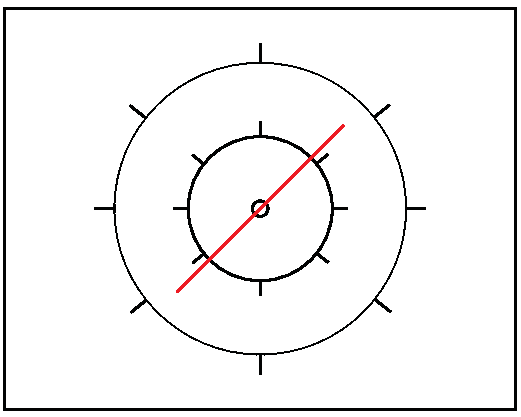
\includegraphics[width=0.33\textwidth]{std_skill_error_1}
\end{center}
\vspace{-20pt}
\caption{50\% Devaluation \label{fig:std_skill_error_1}}
\vspace{-5pt}
\begin{center}
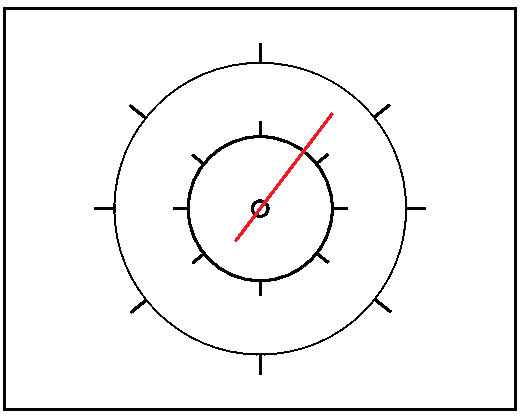
\includegraphics[width=0.33\textwidth]{std_skill_error_2}
\end{center}
\vspace{-20pt}
\caption{100\% Devaluation\label{fig:std_skill_error_2}}
\vspace{-25pt}
\end{wrapfigure}

\textbf{Riding Skills, Repetitive Axis Skills, and Counted Short Skills:} If a figure is broken off in the first half of its required execution, or performed for less than half of the required execution, 100\% is devaluated.
If a figure is broken off in the second half of the required execution, or performed for less than the required execution, 50\% is devaluated.

\textbf{Riding Skills:}
If a rider is not in position for a line figure before crossing the 8-meter circle, but is in position when crossing both 4-meter circle lines, 50\% is devaluated (see figure \ref{fig:std_skill_error_1}).
If the rider is in position but only crosses one edge of the 4-meter circle, 100\% is devaluated (see figure \ref{fig:std_skill_error_2}).

\textbf{Transitions and mounts:} Must finish in the end position (one revolution, $2 \frac{1}{2}$ hops, or $2 \frac{1}{2}$ idles) or 100\% is devaluated.
If the end position for a mount is not defined, must perform one revolution, OR $2 \frac{1}{2}$ hops, OR $2 \frac{1}{2}$ idles before stepping off the unicycle.

\textbf{Axis skills:} If the end position for a axis skill is not defined, must perform one revolution before stepping off the unicycle.
The ending position is not required to be the same as the starting position.

\textbf{Single Short Skills:} Unless otherwise defined in the skill description, the ending position is the same as the starting position.
Must finish in the end position (one revolution, $2 \frac{1}{2}$ hops, or $2 \frac{1}{2}$ idles) or 100\% is devaluated.
If the start and end position for a single short skill is not defined, must perform one revolution, $2 \frac{1}{2}$ hops, OR $2 \frac{1}{2}$ idles before stepping off the unicycle.

\subsection{Start Of Figures}
\oldrule{5.40.4}

All figures start when the rider gets into the position required for that figure.

\subsection{Figure Order}
\oldrule{5.40.5}

Figures left out according to their order on the judging sheet are devaluated 100\%.
This devaluation remains, even if the figure is performed afterward.

\subsection{Figure Patterns}
\oldrule{5.40.5}

Riding figures that the rider doesn't attempt to be ridden as described in section \ref{subsec:freestyle_floor-markings-figure-shapes_riding-area-boundaries} should receive 100\% devaluation.

\textbf{Example:} The line figure is described as ``…start outside the large (8m) circle, cross the center circle, and continue outside the large circle''.
If the rider does not attempt to cross the center circle and performs the line circle completely outside the 4m circle, then 100\% is devaluated.

\section{Execution Devaluations}


\subsection{Wave (~) = -0.5 Point}
\oldrule{5.41.1}

A wave is scored once per skill for each of the following execution mistakes listed below.
More than one wave can be applied to each skill, but if a rider makes the same mistake twice during one skill, they should only receive one wave.

\textbf{Example:} During wheel walking, a rider may have jerky body movements and fingers not together at the beginning – two waves should be applied.
If the rider then smoothly wheel walks for a while and then has jerky body movements again, a third wave should not be applied.
\begin{itemize}
\item insecure entrance or exit 
\item cramped, insecure execution 
\item jerky body movements 
\item not sitting up straight 
\item fingers not together 
\item free leg not stretched, toes not pointed 
\item waving arms 
\item jerky pedal movement 
\item line not straight 
\item circle not round 
\item crossing the 4 m circle when performing a skill in a circle 
\item failure to cross center circle in line or figure 8 
\item circles of figure 8 not the same size 
\item pedal, or foot on pedal touching floor 
\item wandering spin or pirouette 
\item circle size exceeds 1 meter diameter in a spin 
\item going outside riding area boundary 
\item looking at the standard skill order 
\item arms not stretched 
\item arms not horizontal 
\item palms not down 
\item arms touching the body during seat out skills
\end{itemize}

\subsection{Line (/) = - 1 Point}
\oldrule{5.41.2}

A line is scored every time loss of control occurs.
Loss of control includes:
\begin{itemize}
\item loss of proper body form 
\item breaking off and restarting a skill 
\item loss of proper body form before or after transitions
\end{itemize}

\subsection{Cross (+) = - 2 Points}
\oldrule{5.41.3}

A cross is scored each time an unintentional dismount occurs with the competitor landing on his or her feet without the unicycle being dropped.

\subsection{Circle (0) = - 3 Points}
\oldrule{5.41.4}

A circle is scored each time an unintentional dismount occurs with a part of the rider other than his or her feet touching the floor (hand, knee, rear, etc.) or with the unicycle being dropped.
Seat drag skills only have this score applied if a part of the rider other than the feet touches the floor.

\subsection{Applying Lines, Circles, Crosses}
\oldrule{5.41.5}

Lines, circles and crosses are scored every time they occur during and between all skills, whether entered on the score sheet or not.
Only the highest applicable devaluation symbol shall be imposed per execution mistake.
Most waves are not scored if they occur between skills listed on the judging sheet.
Waves can only be scored between skills if they are unrelated to body form.

\textbf{Example:} A competitor will not get a wave if the competitor's arms are not in proper form between skills listed on the judging sheet, but a competitor will get a wave for exceeding the riding area boundary.

\section{Totaling Scores}
\oldrule{5.42}
After the routine is finished, the percentages and symbols from the judges are converted into numbers.
These numbers are subtracted from the rider's starting score.
Then, the scores of the two judging units are added together and divided by two to get the finishing score of a competitor.
The winner in the Standard Skill event is the competitor with the highest score.
If more than one competitor have the same score, placing is decided by the highest Execution score.
If those scores are also the same, the competitors receive tie scores.
